\section{Onion Routing}
\label{onionrouting}
Onion routing is used to ensure sender-receiver anonymity. In contrast
to the Tor-network, there are no exit nodes and the receiver can be anyone
in the onion chain (see fig. \ref{onionrouting}).
\begin{figure}
    \centering
    \caption{Onion Routing}
    \label{onionrouting}
    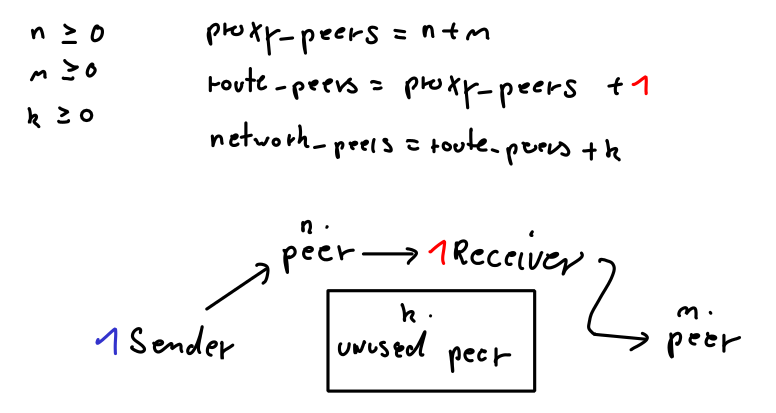
\includegraphics[scale=0.8]{onionrouting.png}
\end{figure}
The peers between the sender and receiver and after the receiver are
called \textit{proxy peers}. The number of proxy peers between the
sender and the receiver and the number of proxy peers after receiver
can range from from 0 up to the maximum number of proxy peers. The sum
of both proxy peers is the \textit{chosen number of proxy peers} and
usually stays consistent for one peer.

The recommended number of proxy peers is \textbf{5}, as a tradeoff between
latency, bandwidth and anonymity. Section \ref{noise}, p. \pageref{noise}
explains in detail why 5 is the recommended number.
% BT: ok
% ----------------------------------------------------------------------------
\subsection{Source Based Routing}
Before creation of an onion, a random route to the receiver is generated.
The route is calculated as follows:
\begin{enumerate}
\item Select random peers from known peer times the number of required proxy peers
\item Shuffle and insert the receiver at a random position
\item Retrieve a random transport protocol address from each peer
\end{enumerate}
For each onion, a new random routes must be calculated.
% ----------------------------------------------------------------------------
\subsection{Onions}
\label{eofonion}
Onions are building the base for the EOF protocol.
The EOF messages described in section \ref{eofmessages}
are multiple times encrypted and assembled according to 
the previously calculated random route. 
The result is called an \textit{onion} and
an example onion is shown in figure \ref{onion}.
\begin{figure}
    \centering
    \caption{An Onion (2 and 3 layers)}
    \label{onion}
    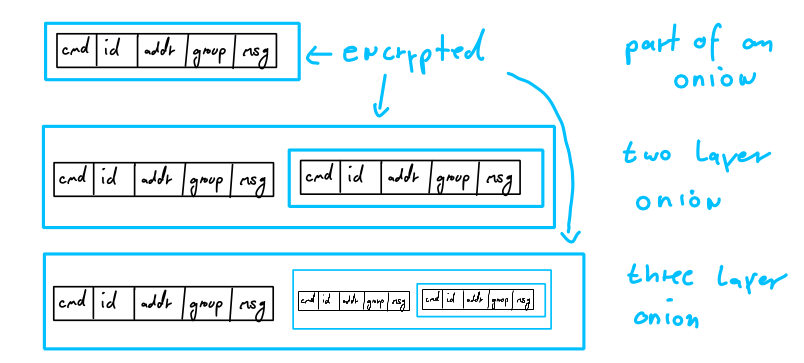
\includegraphics[scale=0.8]{onion.png}
\end{figure}
%% An onion packet is a (multiple times) encrypted packet.
%% An onion packet contains at least one plaintext packet, but can also contain
%% already encrypted packets. It may look like as follows:
Every layer of an onion is encrypted for the specific peer
and the previous encrypted layer is appended after the EOF message
in reencrypted.
In case the onion layer contains the EOF message
3002 or 3003, the layer should also be signed. In all other
cases the onion layer should only be encrypted.
\begin{enumerate}
\item Create EOF message for the last peer
\item Encrypt EOF message for the last peer (first and innermost onion layer)
\item Redo steps one and two for every peer, but append the previous result
\end{enumerate}
% ----------------------------------------------------------------------------
\subsection{Packet Sizes}
The average packet size depending on the number of peers it was
(re-)encrypted for can be found in table \ref{pkgsizes}.
It was generated by running the reference implementation
(\verb=ceof onion -m "test" peer0  | wc -c=)
and increasing the number of proxy peers to be inserted.
The resulting size includes the final onion, 
but does not include transport protocol headers.
\begin{longtable}{|c|c|}
\caption{Packet sizes (experimental)}
\label{pkgsizes}\\
\hline
\textbf{Proxy peers} & \textbf{Packet size (in KiBiBytes)}\\
\hline
\textbf{1} & 1.2\\
\hline
\textbf{2} & 1.9\\
\hline
\textbf{3} & 2.6\\
\hline
\textbf{4} & 3.3\\
\hline
\textbf{5} & 4.0\\
\hline
\textbf{6} & 4.8\\
\hline
\textbf{7} & 5.6\\
\hline
\textbf{8} & 6.3\\
\hline
\textbf{9} & 7.1\\
\hline
\textbf{10} & 8.0\\
\hline
\end{longtable}
